\documentclass[aspectratio=169,t,xcolor=table]{beamer}
\usepackage[utf8]{inputenc}

\usepackage{booktabs} 
\usepackage{subcaption}

\usetheme{Ufg}

%-------------------------------------theorems--------------
\newtheorem{conj}{Conjetura}
\newtheorem{defi}{Definição}
\newtheorem{teo}{Teorema}
\newtheorem{lema}{Lema}
\newtheorem{prop}{Proposição}
\newtheorem{cor}{Corolário}
\newtheorem{ex}{Exemplo}
\newtheorem{exer}{Exercício}

\setbeamertemplate{theorems}[numbered]
\setbeamertemplate{caption}[numbered]

%-------------------------------------------------------------%
%----------------------- Primary Definitions -----------------%

% This command set the default Color, is also possible to choose a custom color
\setPrimaryColor{UFGBlue} 

% First one is logo in title slide (we recommend use a horizontal image), and second one is the logo used in the remaining slides (we recommend use a square image)
\setLogos{lib/logos/infw.png}{lib/logos/infw2.png} 


% -------------------------------------- Title Slide Information
\begin{document}
\title[Inf UFG]{Segmentação Semântica de Nuvens de Pontos LiDAR}
\subtitle{Uma Abordagem Híbrida Combinando Processamento Geométrico
com Aprendizado Profundo}

\author{Matheus Leonel de Andrade\inst{1}}

\institute[UFG] % (optional)
{
  \inst{1}%
  Instituto de Informática\\
  Universidade Federal de Goiás
  \and
}
\date{2025}
%-----------------------The next statement creates the title page.
\frame[noframenumbering]{\titlepage}


%------------------------------------------------Slide 1
\setLayout{vertical} % This command define the layout. 'vertical' can be replace with 'horizontal', 'blank, 'mainpoint', 'titlepage'

\begin{frame}
    \frametitle{Roteiro}
    \tableofcontents
\end{frame}
%---------------------------------------------------------


%---------------------------------------------------------
\section{Introdução}
%---------------------------------------------------------

\setLayout{mainpoint}
\setBGColor{UFGBlue}
\begin{frame}
    \frametitle{Introdução}
\end{frame}
\setLayout{vertical}
\setBGColor{UFGBlue}


\begin{frame}
    \frametitle{Motivação}
    \begin{itemize}
        \item<+-> A percepção 3D do ambiente é um pilar fundamental para sistemas autônomos (veículos autônomos, robótica móvel).
        \item<+-> Sensores LiDAR (Light Detection and Ranging) são essenciais, fornecendo nuvens de pontos 3D densas e precisas.
        \item<+-> \textbf{Desafio:} Processar e interpretar o grande volume de dados das nuvens de pontos (alta dimensionalidade, esparsas, desordenadas) de forma eficiente.
    \end{itemize}
\end{frame}

\begin{frame}
    \frametitle{Problema de Pesquisa}
    \begin{itemize}
        \item<+-> Algoritmos de segmentação e classificação de nuvens de pontos ainda possuem limitações em robustez, escalabilidade e generalização.
        \item<+-> Abordagens baseadas em Deep Learning (e.g., PointNet, KPConv) alcançam alta acurácia, mas exigem alto custo computacional, dificultando o uso em sistemas com recursos limitados.
        \item<+-> A segmentação do solo e a clusterização de objetos são etapas críticas e desafiadoras.
    \end{itemize}
\end{frame}

\begin{frame}
    \frametitle{Objetivos}
    \begin{itemize}
        \item<+-> \textbf{Objetivo Principal:} Desenvolver e avaliar um pipeline eficiente para segmentação e classificação semântica de nuvens de pontos LiDAR.
        \item<+-> \textbf{Abordagem Híbrida:} Combinar a eficiência de métodos clássicos de processamento geométrico com o poder de generalização de técnicas de aprendizado profundo.
        \item<+-> \textbf{Hipótese:} Investigar se a redução da dimensionalidade, através da clusterização, preserva informação semântica suficiente para uma classificação eficaz, equilibrando acurácia e custo computacional.
    \end{itemize}
\end{frame}

%---------------------------------------------------------
\section{Fundamentação Teórica}
%---------------------------------------------------------

\setLayout{mainpoint}
\setBGColor{UFGBlue}
\begin{frame}
    \frametitle{Fundamentação Teórica}
\end{frame}
\setLayout{vertical}
\setBGColor{UFGBlue}

\begin{frame}
    \frametitle{Conceitos Fundamentais}
    \begin{columns}[T]
       \begin{column}{.5\textwidth}
            \begin{block}{Nuvens de Pontos 3D}
                \begin{itemize}
                    \item<+-> Conjunto de pontos com coordenadas (x, y, z).
                    \item<+-> Representação direta da geometria da cena.
                    \item<+-> Dados não estruturados, esparsos e com densidade variável.
                    \item<+-> LiDAR gera padrão de "scanlines".
                \end{itemize}
            \end{block}
        \end{column}
        \begin{column}{.5\textwidth}
            \begin{block}{Segmentação e Clusterização}
                \begin{itemize}
                    \item<+-> \textbf{Segmentação:} Atribuir um rótulo semântico a cada ponto (e.g., solo, carro, prédio).
                    \item<+-> \textbf{Clusterização:} Agrupar pontos próximos que pertencem ao mesmo objeto físico.
                \end{itemize}
            \end{block}
        \end{column}
    \end{columns}
\end{frame}


%---------------------------------------------------------
\section{Metodologia}
%---------------------------------------------------------

\setLayout{mainpoint}
\setBGColor{UFGBlue}
\begin{frame}
    \frametitle{Metodologia}
\end{frame}
\setLayout{vertical}
\setBGColor{UFGBlue}

\begin{frame}
    \frametitle{Pipeline Proposto}
    \begin{figure}
        \centering
        % Placeholder text instead of image
        \fbox{
            \begin{minipage}{0.9\textwidth}
                \centering
                \textbf{1. Nuvem de Pontos Bruta (Entrada)} \\
                $\downarrow$ \\
                \textbf{2. Pré-processamento} \\
                (GPF para Segmentação do Solo + SLR para Clusterização) \\
                $\downarrow$ \\
                \textbf{3. Extração de Características por Cluster} \\
                $\downarrow$ \\
                \textbf{4. Classificação com PointNet (Saída)}
            \end{minipage}
        }
    \end{figure}
\end{frame}

\begin{frame}
    \frametitle{Dataset: SemanticKITTI}
    \begin{itemize}
        \item<+-> Benchmark de referência para percepção 3D em condução autônoma.
        \item<+-> Extensão semântica do KITTI Vision Benchmark.
        \item<+-> Fornece anotações semânticas densas para nuvens de pontos capturadas por um LiDAR Velodyne HDL-64E.
        \item<+-> Foco do trabalho em 20 classes semânticas relevantes para navegação.
    \end{itemize}
\end{frame}

\begin{frame}
    \frametitle{Dataset: SemanticKITTI}
    \begin{figure}
        \centering
        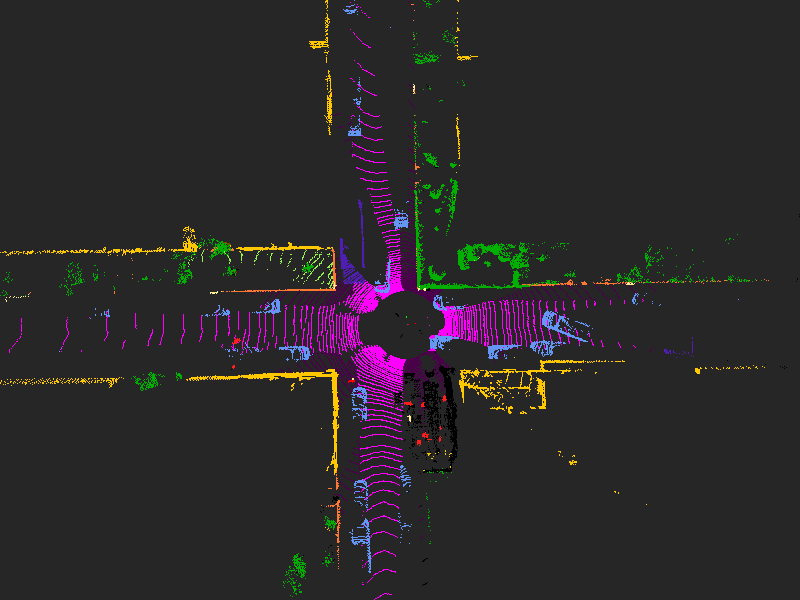
\includegraphics [width=0.5\textwidth]{figs/final-true1t.png}
        \caption {Exemplo de uma cena do SemanticKITTI com rótulos semânticos.}
    \end{figure}
\end{frame}

\begin{frame}
    \frametitle{Pré-processamento: Segmentação do Solo (GPF)}
    \begin{columns}[T]
        \begin{column}{.4\textwidth}
            \begin{block}{Objetivo}
                \vspace{1.5em}
                Identificar e remover os pontos pertencentes ao solo.
                \vspace{1.5em}
            \end{block}
            \begin{block}{Algoritmo}
                \vspace{1.5em}
                Ground Plane Fitting (GPF).
                \vspace{1.5em}
            \end{block}
        \end{column}
        \begin{column}{.6\textwidth}
            \begin{block}{Como funciona}
                \begin{enumerate}[<+->]
                    \item A nuvem de pontos é dividida em setores angulares.
                    \item Em cada setor, o solo é modelado como um plano.
                    \item O plano é estimado de forma iterativa usando SVD sobre os pontos de menor altura.
                    \item Pontos próximos ao plano estimado são classificados como solo.
                \end{enumerate}
            \end{block}
        \end{column}
    \end{columns}
\end{frame}

\begin{frame}
    \frametitle{Pré-processamento: Clusterização de Objetos (SLR)}
    \begin{columns}[T]
        \begin{column}{.4\textwidth}
            \begin{block}{Objetivo}
                \vspace{1.5em}
                Agrupar os pontos remanescentes (não-solo) em clusters que representam objetos.
                \vspace{1.5em}
            \end{block}
            \begin{block}{Algoritmo}
                \vspace{1.5em}
                Scan Line Run (SLR).
                \vspace{1.5em}
            \end{block}
        \end{column}
        \begin{column}{.6\textwidth}
            \begin{block}{Como funciona}
                \begin{enumerate}[<+->]
                    \item Explora a estrutura sequencial das scanlines do LiDAR.
                    \item Pontos em uma mesma scanline são agrupados com base na proximidade.
                    \item Clusters de scanlines adjacentes são fundidos se estiverem próximos.
                    \item Resultado: Uma lista de clusters, cada um representando um potencial objeto.
                \end{enumerate}
            \end{block}
        \end{column}
    \end{columns}
\end{frame}

%---------------------------------------------------------
\section{Resultados}
%---------------------------------------------------------

\setLayout{mainpoint}
\setBGColor{UFGBlue}
\begin{frame}
    \frametitle{Resultados}
\end{frame}
\setLayout{vertical}
\setBGColor{UFGBlue}

\begin{frame}
    \frametitle{Avaliação do Pré-processamento}
    \begin{columns}[T]
        \begin{column}{.5\textwidth}
            \begin{alertblock}{Redução de Dimensionalidade}
                O pipeline reduziu o número de pontos em \textbf{98,84\%}.
            \end{alertblock}
            \begin{itemize}
                \item<2-> Transforma uma nuvem com $\sim$120.000 pontos em $\sim$1.400 clusters.
                \item<2-> Redução massiva do custo computacional para a etapa de classificação.
            \end{itemize}
            \vspace{1cm}
            \begin{alertblock}{Consistência Semântica}
                \textbf{95\%} dos clusters gerados eram "semanticamente puros".
            \end{alertblock}
            \begin{itemize}
                \item<3-> Indica que a clusterização geométrica preserva a separação semântica dos objetos.
            \end{itemize}
        \end{column}
        \begin{column}{.5\textwidth}
            \begin{figure}
                \includegraphics<4->[width=\textwidth]{figs/cluster_1_s4f75.png}
                \caption<4->{Clusters (cores aleatórias).}
            \end{figure}
            \begin{figure}
                \includegraphics<4->[width=\textwidth]{figs/label_1_s4f75.png}
                \caption<4->{Rótulos verdadeiros.}
            \end{figure}
        \end{column}
    \end{columns}
\end{frame}

\begin{frame}
    \frametitle{Resultados da Classificação}
    \begin{itemize}
        \item<+-> Após o pré-processamento, um vetor de características foi extraído para cada cluster.
        \item<+-> Uma rede PointNet simplificada foi usada para classificar cada cluster.
    \end{itemize}
    \begin{alertblock}{Acurácia de Classificação}
        O modelo alcançou \textbf{93,27\%} de acurácia na classificação dos clusters.
    \end{alertblock}
    \begin{itemize}
        \item<+-> \textbf{Conclusão:} A representação compacta em clusters, mesmo após uma redução de dados de >98\%, reteve informação suficiente para uma classificação semântica de alta qualidade.
    \end{itemize}
    \begin{figure}
        \centering
        \includegraphics<+->[width=0.6\textwidth]{figs/plot-1.png}
        \caption<+->{Matriz de confusão normalizada (exemplo).}
    \end{figure}
\end{frame}

%---------------------------------------------------------
\section{Conclusão e Trabalhos Futuros}
%---------------------------------------------------------

\setLayout{mainpoint}
\setBGColor{UFGBlue}
\begin{frame}
    \frametitle{Conclusão e Trabalhos Futuros}
\end{frame}
\setLayout{vertical}
\setBGColor{UFGBlue}

\begin{frame}
    \frametitle{Conclusões}
    \begin{itemize}
        \item<+-> O trabalho validou um pipeline híbrido que combina processamento geométrico clássico com aprendizado profundo para segmentação semântica de nuvens de pontos.
        \item<+-> A abordagem demonstrou um excelente equilíbrio entre eficiência computacional e acurácia.
    \end{itemize}
    \begin{alertblock}{Principal Contribuição}
        Demonstração de que é possível comprimir drasticamente nuvens de pontos LiDAR em representações de clusters, preservando a informação semântica essencial para a classificação.
    \end{alertblock}
    \begin{itemize}
        \item<+-> Os resultados (redução de 98.8\%, acurácia de 93.3\%) confirmam a viabilidade da metodologia para aplicações que demandam eficiência.
    \end{itemize}
\end{frame}

\begin{frame}
    \frametitle{Limitações e Trabalhos Futuros}
    \begin{columns}[T]
        \begin{column}{.5\textwidth}
            \textbf{Limitações}
            \begin{itemize}
                \item<+-> Propagação de erros: falhas na segmentação do solo afetam a clusterização e classificação.
                \item<+-> A clusterização pode fragmentar objetos grandes ou complexos.
                \item<+-> Validação restrita ao dataset SemanticKITTI.
                \item<+-> Implementação não otimizada para tempo real.
            \end{itemize}
        \end{column}
        \begin{column}{.5\textwidth}
            \textbf{Trabalhos Futuros}
            \begin{itemize}
                \item<+-> Aprimorar a segmentação do solo (modelos mais flexíveis).
                \item<+-> Enriquecer as características dos clusters (e.g., intensidade, contexto).
                \item<+-> Otimizar o pipeline para hardware embarcado.
                \item<+-> Validar em outras plataformas robóticas e com diferentes sensores.
            \end{itemize}
        \end{column}
    \end{columns}
\end{frame}

%---------------------------------------------------------
\setLayout{blank}
\begin{frame}
    \centering
    \vspace{3cm}
    
    \textbf{\Huge Obrigado!}
    
    \vspace{1cm}
    
    \textbf{\Large Perguntas?}
    
    \vspace{3cm}
    \begin{figure}
        \centering
        \begin{subfigure}{0.2\textwidth}
            \centering
            
\includegraphics[height=1.5cm]{lib/logos/infw.png}
        \end{subfigure}%
        \qquad 
        \begin{subfigure}{0.2\textwidth}
            \centering
            
\includegraphics[height=1.5cm]{lib/logos/ufgw.png}
        \end{subfigure}
    \end{figure}
\end{frame}

\end{document}